\medskip

\textbf{Partie A.}

\medskip



\begin{enumerate}
	\item Un arbre de probabilité représentant la situation est :

	\hfill~
	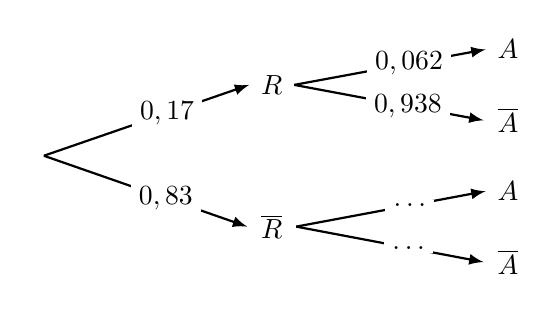
\begin{tikzpicture}[xscale=1,yscale=1,baseline={(R.base)}]
		\tikzstyle{fleche}=[->,>=latex,thick]
		\tikzstyle{noeud}=[fill=white,circle,inner sep=2pt]
		\tikzstyle{feuille}=[fill=white,circle,inner sep=2pt]
		\tikzstyle{etiquette}=[pos=0.6,fill=white, inner xsep=3pt, inner ysep=1.5pt]
		\def\DistanceInterNiveaux{3}
		\def\DistanceInterFeuilles{0.9}
		\def\NiveauA{(0)*\DistanceInterNiveaux}
		\def\NiveauB{(1)*\DistanceInterNiveaux}
		\def\NiveauC{(2)*\DistanceInterNiveaux}
		\def\InterFeuilles{(-1)*\DistanceInterFeuilles}
		
		\node[noeud] (R) at ({\NiveauA},{(1.5)*\InterFeuilles}) {};
		\node[noeud] (Ra) at ({\NiveauB},{(0.5)*\InterFeuilles}) {$R$};
		\node[feuille] (Raa) at ({\NiveauC},{(0)*\InterFeuilles}) {$A$};
		\node[feuille] (Rab) at ({\NiveauC},{(1)*\InterFeuilles}) {$\overline{A}$};
		\node[noeud] (Rb) at ({\NiveauB},{(2.5)*\InterFeuilles}) {$\overline{R}$};
		\node[feuille] (Rba) at ({\NiveauC},{(2)*\InterFeuilles}) {$A$};
		\node[feuille] (Rbb) at ({\NiveauC},{(3)*\InterFeuilles}) {$\overline{A}$};
		
		\draw[fleche] (R.east)--(Ra.west) node[etiquette] {$0,17$};
		\draw[fleche] (Ra.east)--(Raa.west) node[etiquette] {$0,062$};
		\draw[fleche] (Ra.east)--(Rab.west) node[etiquette] {$0,938$};
		\draw[fleche] (R.east)--(Rb.west) node[etiquette] {$0,83$};
		\draw[fleche] (Rb.east)--(Rba.west) node[etiquette] {$\ldots$};
		\draw[fleche] (Rb.east)--(Rbb.west) node[etiquette] {$\ldots$};
	\end{tikzpicture} \hfill~


\item
	\begin{enumerate}
		\item $P(R\cap A) = P(R)\times P_R(A)= 0,17\times 0,062= \np{0,01054}$

La probabilité que l'enfant interrogé habite en zone rurale et soit atteint d'allergie alimentaire vaut $ \np{0,01054}$.

		\item Les évènements $R$ et $\overline{R}$ forment une partition de l'univers, donc, d'après la formule des probabilités totales : \quad $P(A) = P\big(\,R\cap A\big) + P\big(\,\overline{R}\cap A\big) $

On a donc : \quad $0,09 = 0,01054 +P\big(\,\overline{R}\cap A\big) $

D'où  $P\big(\,\overline{R}\cap A\big) = 0,09-\np{0,01054}=\np{0,07946}$

La probabilité que l'enfant interrogé habite en zone urbaine et soit atteint d'allergie alimentaire vaut $\np{0,07946}$.

		\item $P_{\overline{R}}(A)=\dfrac{P\big(\,\overline{R}\cap A\big)}{P\left(\overline{R}\right)}= \dfrac{\np{0,07946}}{0,83}= \dfrac{\np{3973}}{\np{41500}}\approx \np{0,09573}$.

La probabilité qu'un enfant  soit atteint d'allergie alimentaire sachant qu'il habite en zone urbaine vaut $\np{0,0957}$ arrondi à $10^{-4}$.
	\end{enumerate}
\end{enumerate}

\smallskip

\textbf{Partie B.}

\medskip

\begin{enumerate}
\item On répète 100 fois de manière identique et indépendante une expérience aléatoire à deux issues dont le succès \og L'enfant est atteint d'une allergie alimentaire \fg{}  a une probabilité $p = 0,09$.

La variable aléatoire $X$ compte le nombre de succès.

Donc $X$ suit une loi binomiale de paramètres $n=100$ et $p = 0,09$.
\item À l'aide de la calculatrice : $P(X \geqslant 10)\approx \np{0,41249}$

La probabilité qu'au moins 10 enfants parmi les 100 interrogés soient atteints d'allergie alimentaire vaut $\np{0,4125}$ arrondi à $10^{-4}$.
\end{enumerate}

\smallskip

\textbf{Partie C.}

\medskip

\begin{enumerate}
	\item Dans le contexte de l'exercice, la variable aléatoire $M_{20}$ représente l'âge moyen d'apparition des premiers symptômes pour les 20 enfants.
	\item  $M_{20}$ est la moyenne d'un échantillon de taille $n$ d'une variable aléatoire $A$ telle que $E(A)=4$ et $V(A)=2,25$ d'où :

$E\left(M_{20}\right) = E(A)= 4$


$V\left(M_{20}\right) = \dfrac{V(A)}{20}=\dfrac{2,25}{20} = \np{0,1125}$

	\item L'évènement \og $2<M_{20}< 6$ \fg{} revient à 
	
$\big|M_{20} - 4 \big| < 2$ et $P\Big(\big|M_{20} - 4 \big| < 2\Big) = 1 - P\Big(\big|M_{20} - 4 \big| \geqslant 2\Big)$.

Or, d'après l'inégalité de concentration, pour tout réel $t > 0$ : 

$P\Big(\big|M_n - E(A)\big| \geqslant t \Big) \leqslant \dfrac{V(A)}{nt^2}$.

Soit ici, avec $n=20$ et $t =2$ : $P\Big(\big|M_{20} - 4 \big| \geqslant 2\Big) \leqslant \dfrac{2,25}{20 \times 2^2}$,

d'où \[
\begin{aligned}
P\left( \left| M_{20} - 4 \right| < 2 \right)
&\geqslant 1 - \frac{\operatorname{Var}(M_{20})}{2^2} \quad \text{(inégalité de Bienaymé-Tchebychev)} \\
P\left( \left| M_{20} - 4 \right| < 2 \right)&= 1 - \frac{2,25}{80} \\
P\left( \left| M_{20} - 4 \right| < 2 \right)&= \frac{311}{320}
\end{aligned}
\]

Or $\dfrac{311}{320}\approx \np{0,9719}$,

donc : $ P(2 < M_{20} < 6) > 0,97.$

Dans le contexte de l'exercice cela signifie que dans plus de 97\,\% des cas, les premiers symptômes apparaissent entre 2 et 6 ans.
\end{enumerate}

\medskip
